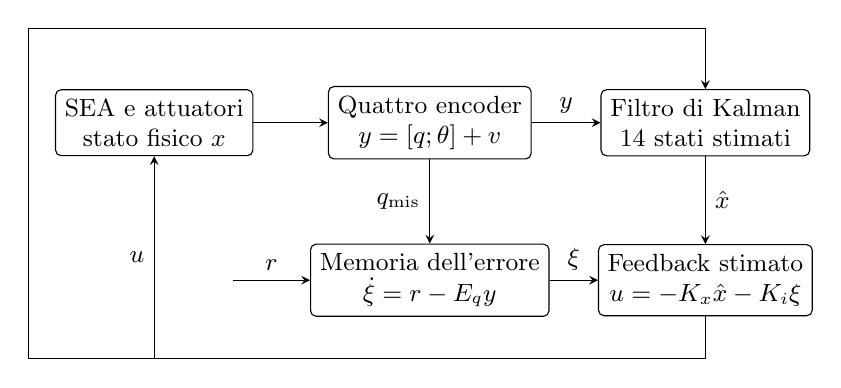
\begin{tikzpicture}[font=\small,>=stealth,
  block/.style={draw,rounded corners=2pt,minimum width=2.2cm,minimum height=.8cm,align=center}]
\node[block] (plant) at (0,0) {SEA e attuatori\\stato fisico $x$};
\node[block] (sensors) at (3.5,0) {Quattro encoder\\$y=[q;\theta]+v$};
\node[block] (kalman) at (7,0) {Filtro di Kalman\\14 stati stimati};
\node[block] (feedback) at (7,-2) {Feedback stimato\\$u=-K_x\hat x-K_i\xi$};
\node[block] (integral) at (3.5,-2) {Memoria dell'errore\\$\dot\xi=r-E_qy$};
\draw[->] (plant)--(sensors);
\draw[->] (sensors)--node[above] {$y$} (kalman);
\draw[->] (kalman)--node[right] {$\hat x$} (feedback);
\draw[->] (sensors)--node[left] {$q_{\rm mis}$} (integral);
\draw[->] (integral)--node[above] {$\xi$} (feedback);
\draw[->] (1,-2)--node[above] {$r$} (integral);
\draw[->] (feedback.south)--(7,-3)--(0,-3)--node[left] {$u$} (plant.south);
\draw[->] (0,-3)--(-1.6,-3)--(-1.6,1.2)--(7,1.2)--(kalman.north);
\end{tikzpicture}
